We apply our method to Zynga Inc's strategy game called ``Empires and Allies''.
In the game, the goal is to conquer all the battlefields
in a global map,  either with machine or with other players. To conquer 
the battles, the players need to build/upgrade base resources such as weapons and troops, which in turn 
requires game points that can be obtained from winning battles.  Thus, the players need to 
tradeoff between building resources and conquering battlefields.

%We apply our method to one of Zynga Inc's mobile strategy game -- Empires and Allies, an all-new modern military strategy game that players can design their army, build their base and deploy their weapons and troops to conquer the battlefields. Thanks to the powerful backend system, the game tracks almost every action each player does in the game, which provide us a handful data set to investigate the sophisticated player types. We choose a data set which contains a daily active cohort's 10 consecutive days data from the first day they install the game. For each player and each day, we have 67 features including engagement features like session length, number of battles, game action features like deploy a tank, build a defence building and join an alliance. Then we use the feature selection algorithm to choose 5 out of 67 features to build the time series clustering model. They are PvP (People vs People) Battle , PvE (People vs Bot) Battle, Points gained/lost per battle, session length, Level up and is-Payer.  

We form a dataset that contains player's 10 consecutive days data after installation, 
and subsample users that are active at all the 10 days. This results in 1719 players.
Each player is measured with $67$ metrics at each day, and we select $5$ important 
features based on prior experience: \texttt{PvP} (people vs people battle), 
\texttt{Pve} (people vs machine battle), \texttt{Points} (number of points gained), \texttt{Session} 
(number of session started), \texttt{LevelUp} (whether a player level up) and \texttt{isPayer} (whether
the player paid). We model \texttt{Points}  with Gaussian distribution, \texttt{Session} with
Poisson distribution, and the rest features with Bernoulli distribution.


%\begin{wrapfigure}{r}{0.4\textwidth}
%\centering
%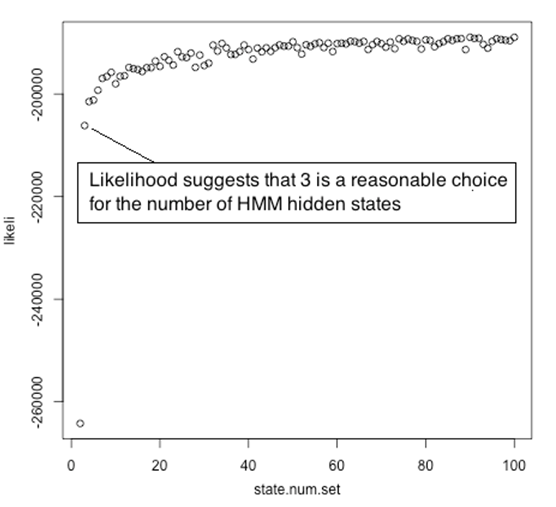
\includegraphics[width=0.35\textwidth]{likeli} 
%\caption{Data likelihood using different number of playing states.}
%\label{fig:likeli}
%\end{wrapfigure}




\subsection{Identifying Players' Daily States}
We fit HMM model with different number of playing states and found that 3 states is reasonable. 
%Figure \ref{fig:likeli} plots the data likelihood using different number of playing states. 
%From the results, we see that using 3 hidden states is reasonable for explaining our data. 
Table \ref{tab:states} lists the discovered playing states, \textbf{Aggressive}, 
\textbf{Defensive}, and \textbf{Moderate}.  The \textbf{Aggressive} state captures 
the mode where the players focus on conquering battles, while the \textbf{Defensive} 
state describes the stage that they build the resources. The \textbf{Moderate} is a mixture
of the two. These states interestingly identified the design of the game explained previously,
namely, the players have to conquer battles and build resources intermittently in order to improve. 
\begin{wraptable}{r}{8.2cm}
\caption{Discovered Playing States}
\label{tab:states}
\centering
\begin{tabular}{lccc} 
\bf Feature / State & \textbf{Aggressive}  & \textbf{Defensive}  &  \textbf{Moderate} 
\\ \hline \\
 Prob.\ \texttt{Pvp}     &  0.2472  & 0.0295 &  0.0947  \\
 Prob.\ \texttt{Pve}     &  0.2430  & 0.0581 &  0.1044 \\
 Mean \texttt{Points} &  88.10   & 1238.36 &  476.22 \\
 Mean \texttt{Session}&  4.58    &  34.19  & 12.95 \\
 Prob.\ \texttt{LevelUp} &  0.1664  & 0.0177  & 0.0553 \\
 Prob.\ \texttt{Pay}     &  0.0031  & 0.0956  & 0.0320 \\
\end{tabular}
\end{wraptable}

We then decode player's  states at each day.
Figure \ref{fig:transitions} plots the transitions for all the users among the 10 days. 
The result shows that most of the users starts with the \textbf{Moderate} or \textbf{Defensive} state, 
and then gradually transition to the \textbf{Aggressive} state. 
This is also consistent with the game design since the players can not start with many battles at
the beginning due to the resources restriction, but they ultimately need to 
conquer all the battlefields.

\begin{figure}[h]
\begin{minipage}[b]{0.3\linewidth}
    \centering
    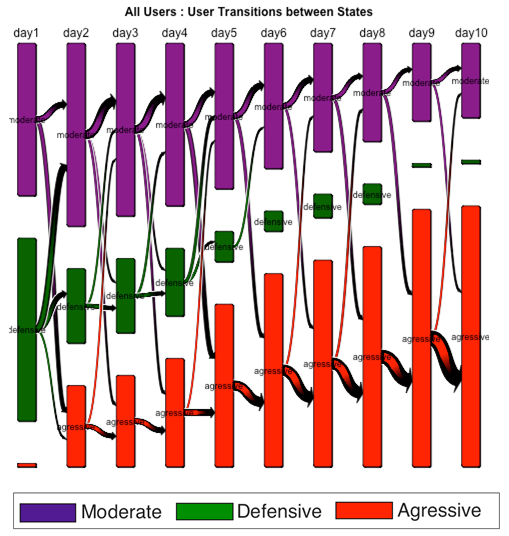
\includegraphics[width=0.8\linewidth]{transitions} 
    \caption{State transitions of all the Players at the first 10 days of installing the game.}
    \label{fig:transitions}
\end{minipage}
\quad
\begin{minipage}[b]{0.65\linewidth}
    \centering
        \begin{tabular}{ccc}
         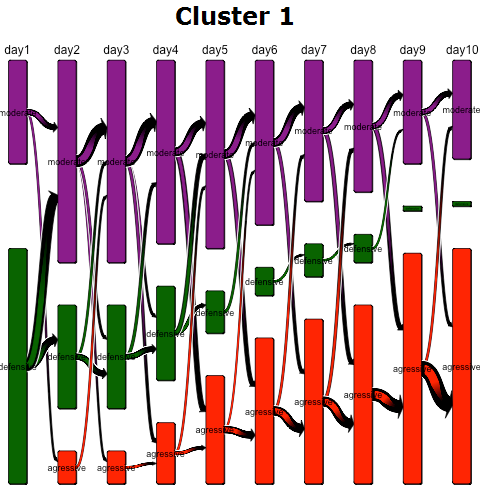
\includegraphics[width=0.33\textwidth]{cluster1} &
         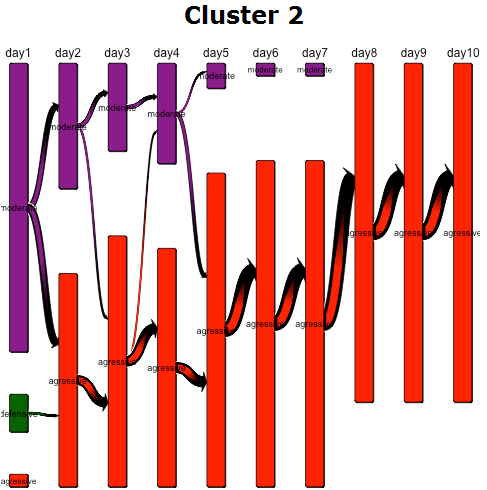
\includegraphics[width=0.33\textwidth]{cluster2} &
         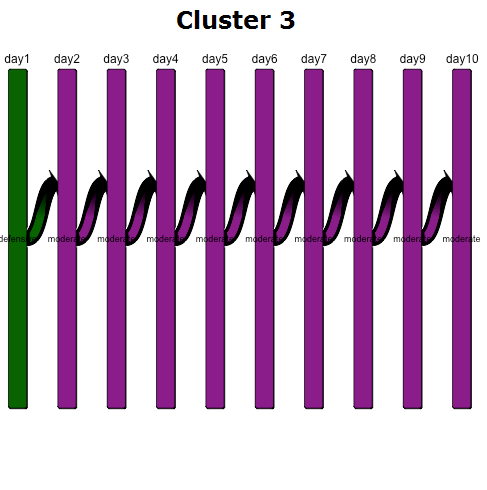
\includegraphics[width=0.33\textwidth]{cluster3} \\
         \multicolumn{3}{c}{ 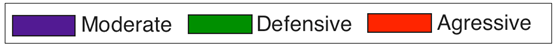
\includegraphics[width=0.8\textwidth]{legend} }
         \end{tabular}
     \caption{\label{fig:clusters} State transitions within three clusters found by our method.}
\end{minipage}
\end{figure}

%
%\begin{table}[t]
%\caption{Discovered Playing States}
%\label{tab:states}
%\centering
%\begin{tabular}{ccccccc}
%\bf State & \bf Pvp Pr. & \bf Pve Pr. & \bf Points Mean & \bf Session Mean & \bf LevelUp Pr. & \bf Pay Pr. 
%\\ \hline \\
%\texttt{Aggressive} & 0.2472  &  0.2430  &  88.10   &  4.58   & 0.1664  & 0.0031 \\  
%\texttt{Defensive}  & 0.0295  &  0.0581  &  1238.36 &  34.19  & 0.0177  & 0.0956 \\
%\texttt{Moderate}   & 0.0947  &  0.1044  &  476.22  &  12.95  & 0.0553  & 0.0320 
%\end{tabular}
%\end{table}


%\begin{figure}[t]
%\centering
%    \begin{tabular}{ccc}
%     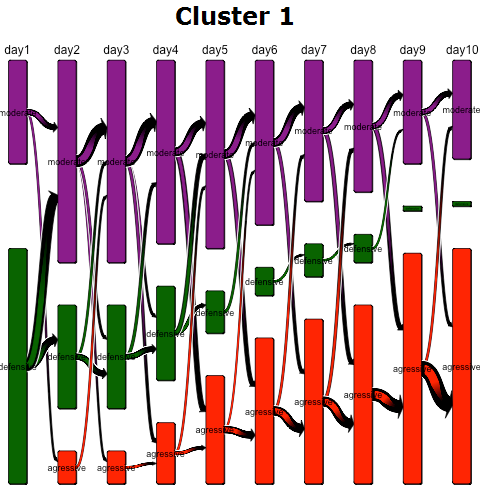
\includegraphics[width=0.26\textwidth]{cluster1} &
%     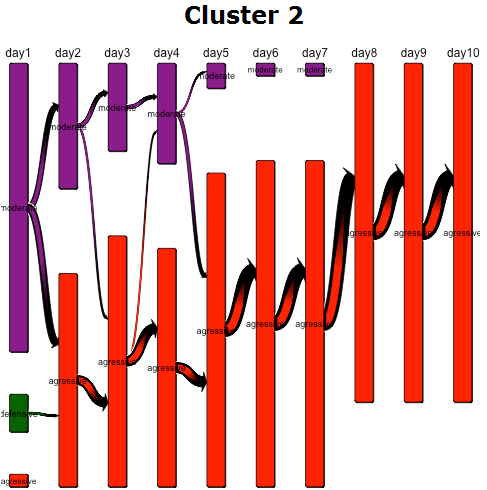
\includegraphics[width=0.26\textwidth]{cluster2} &
%     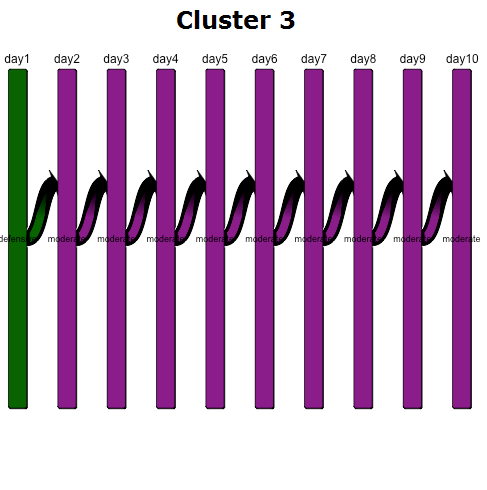
\includegraphics[width=0.26\textwidth]{cluster3} \\
%     \multicolumn{3}{c}
%      { 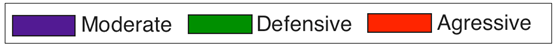
\includegraphics[width=0.45\textwidth]{legend} }
%    \end{tabular}
%     \caption{\label{fig:clusters} State transitions within the three clusters found by our method.
%              }
%\end{figure}
%
\subsection{Clustering Results}
Next we clustering users based on their state transitions with the method explained in Sec.\ \ref{sec:clustering} . 
\begin{wraptable}{r}{4.5cm}
\caption{Clustering results.}
\label{tab:clustering}
\begin{tabular}{ccc}
\bf Method & \bf \#Cluster & \bf DB
\\ \hline \\
{\bf Our}     & {\bf 3}  &  {\bf 0.968} \\  
Kmeans  &  5  &  2.628 \\
GMM     &  4  &  1.803 
\end{tabular}
\end{wraptable} 
We compare with two baselines: Kmeans and Gaussian Mixture Model (GMM). 
Due to the fact that we do not have actual cluster labels, we evaluate the results using a polular
internal evaluation method Davis-Bouldin (DB) index \cite{dbindex}. 
We tune the number of clusters for Kmeans using DB index, and report the one that has the best (the smallest) DB index value. 
Table \ref{tab:clustering} report the clustering results of all methods, 
where our method outperforms the baselines. We also plot the state transitions within each clusters  
and found that our method produces the most meaningful results. Here we show the within cluster transitions found by our
method at Figure \ref{fig:clusters}.  


